\chapter{The $\alpha$-shapes approach to compute the boundaries in target phase space}\label{chap:boundaries_alpha}
The $\alpha$-shape method which is widely used for reconstruction an unknown surface from a set of data points, \cite{guo1997surface}.
We develop a technique based on $\alpha$-shape to obtain an approximation of the boundaries of the set of points obtained from the triangulation refinement.
The aim is to give a criterion to determine the value of the parameter $\alpha$ that gives the better approximation of the boundaries.
The results are given in Section \ref{sec:Tir_alpha} for two different kind of total internal reflection (TIR) collimator.
\section{The $\alpha$-shapes approach}
In this paragraph we give an overview of the state of art about $\alpha$-shapes methods.
Given a finite set $V$ of points $\alpha$-shapes are geometrical objects that give us an approximation of the shape\footnote{It will become clear through this chapter what we intend with the word \textit{shape}.} formed by the points in $V$.\\ \indent
Before giving a formal definition, we explain an intuitive and nice interpretation of $\alpha$-shapes, \cite{lucieer2004alpha}. 
We can think to a mass of a stracciatella ice-cream\footnote{Stracciatella ice cream is made with milk-based ice-cream and fine peaces of chocolate, \cite{Wiki3}.}. If we desire to know the shape formed by the chocolate pieces we can start eating the ice cream using a spoon with a spherical shape and trying to do not remove any piece of chocolate. 
We will obtain a shape formed by arcs and points, see Figure \ref{fig:shape2d} for the two-dimensional case.
\begin{figure}[htbp]\label{fig:shape2d}
\begin{center}
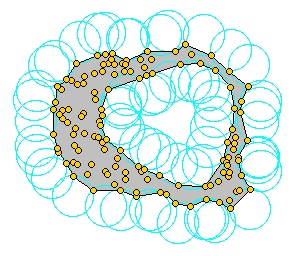
\includegraphics[width=7cm]{shape.jpg}
\label{fig:shape}
\caption{Construction of $\alpha$-shape given a set of points in $\mathbb{R}^2$}
\label{fig:shape2d}
\end{center}
\end{figure}
Straightening the arcs to line segments we obtain broken lines which constitute the boundaries of the so-called $\alpha$-shape formed by the points of the points set $V$. In this example, the chocolates peaces are the points of $V$ and, the parameter $\alpha$ determines the radius of the carving spoon (the spherical spoon in two-dimension is simply a circle). A very small spoon will allow us to eat the entire ice cream without eating any piece of chocolate, while with a huge spoon we are not able to eat any part of the ice cream because we will always take away at least one chocolate peace.\\ \indent 
The previous example might give a better understanding of the definition of $\alpha$-shape first given by Edelsbrunner, Kirkpatrick and Seidel in 1983, \cite{edelsbrunner1983shape}. They describe $\alpha$-shape has a generalization of the convex hull of a finite set of point in the plane. Let be $\alpha$ a not negative number $0\leq\alpha<\infty$. 
If $\alpha$ is equal to $0$ the shape degenerates to the point set $V$. On the other hand, when $\alpha\rightarrow\infty$ the $\alpha$-shape is simply the convex hull of $V$. If $0<\alpha<\infty$ the $\alpha$-shape is a polytope of $V$, \cite{edelsbrunner1994three}. The construction of $\alpha$-shape is closely related to Delaunay triangulation of $V$,\cite{mucke1993shapes}. Therefore, a formal definition of triangulations and Delanauy triangulations is now required. \\ \indent
Given a set $V$ of not all aligned points, let us consider the set $E$ of all the straight line segments whose endpoints are in $V$. 
A triangulation $T$ of $V$ is the maximum subset of $E$ such that all the line segments of $T$ intersect only at their endpoints, \cite{lloyd1977triangulations}. \\ \indent 
The Delaunay triangulation of the points set $V$ has the property (called Delaunay property) that the circle circumscribed by any triangle of $T$ does not contain any point of $V$. A very common used algorithm to construct such triangulation is explained in the following. 
A Delaunay triangulation is constructed by modifying a general triangulation $T$ such that every point satisfies the Delaunay property. 
Therefore, every triangle (or tetrahedron in three dimensions) that does not satisfy such property is flipped such that the new edge is part of the triangulation, see Figure \ref{fig:Delaunay}. 
More precisely, given an arbitrary triangulation $T$ in two-dimension, for each edge $\bar{ab}$ in $T$ which is not on the boundary of the convex hull the two triangles 
$\Delta_{abc}$ and $\Delta_{abd}$ with the common edge $\bar{ab}$ are found. Then, if either the circumcircle of triangle $\Delta_{abc}$ contains point $d$ or the circumcircle of triangle $\Delta_{abd}$ contains point $c$ the edge $\bar{ab}$ cannot be included in the Delaunay triangulation and, therefore, it is flipped such that the other two possible triangles $\Delta_{acd}$ and $\Delta_{bcd}$ are found. The new edge $\bar{cd}$ satisfy the Delaunay property locally and the triangles are added to the Delaunay triangulation.  
\begin{figure}[h]\label{fig:Delaunay}
\begin{center}
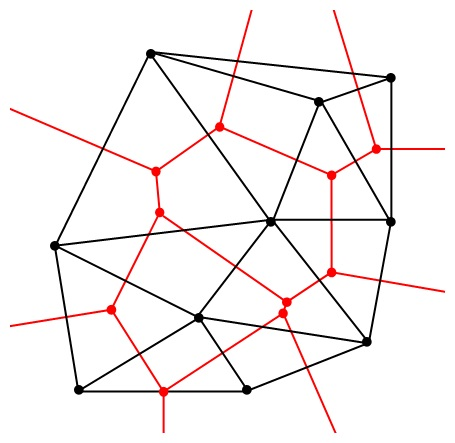
\includegraphics[width=7cm]{Delaunay_Voronoi.jpg}
\label{fig:shape}
\caption{Triangles flipped.}
\label{fig:Delaunay}
\end{center}
\end{figure}
Several others algorithm have been developed to construct a Delaunay triangulation, see for example \cite{lee1980two, renka1997algorithm}.
The Delaunay triangulation $T^\prime$ derived from a triangulation $T$ of a given points set $V$ is unique. It has the property to have the largest minimum angle among all possible triangulation of a point set $V$, \cite{press2007numerical}. 
Delaunay triangulation can be seen as the dual of Voronoi diagram, \cite{fortune1992voronoi}.\\\indent
We give here the definition of Voronoi diagram in two dimensions, (see \cite{brown1979voronoi} for higher dimensions).
In every finite set of point $V = \{v_1, \cdots, v_N\}\subset \mathbb{R}^2$ and for \textit{almost}\footnote{It is needed to specify the word \textit{almost} because some points can have the same distance with two or more points of $V$.} every point $x\in \mathbb{R}^2$, there is a point which is the closest point to $x$. The Voronoi cell of a point $v_\variabile{i}\in V$ contains all points in $\mathbb{R}^2$ which are closer to $v_{\variabile{i}}$, see Figure {fig:Voronoi}. 
The Voronoi diagram is the set of all Voronoi cells, \cite{cazals2005conformal}.
A formal definition of the Voronoi diagram is given in the following.
\begin{defn}
Let $X$ be a metric space with a distance $\textrm{d}$ and $V=\{v_1,\cdots,v_N\}$ a set of point in $X$. The Voronoi cell $V_\variabile{i}$ associated with the point $v_\variabile{i}$ with $v_{\variabile{i}}\in\{1,\cdots,N\}$ is defined as:
\begin{equation}
V_\variabile{i}=\{x\in X\; | \;\textrm{d}(x,v_\variabile{i})\leq \textrm{d}(x,v_\variabile{j}) \quad \forall \variabile{j}\neq \variabile{i} \}\,,
\end{equation}
The Voronoi diagram is defined as the union $U = \bigcup_{\variabile{i}=1}^N V_\variabile{i}$ where $V_{\variabile{i}}\cap V_{\variabile{j}}= \emptyset$ for $\variabile{i}\neq\variabile{j}$.
\end{defn}
Figure \ref{fig:Voronoi}
\begin{figure}[h]\label{fig:Voronoi}
\begin{center}
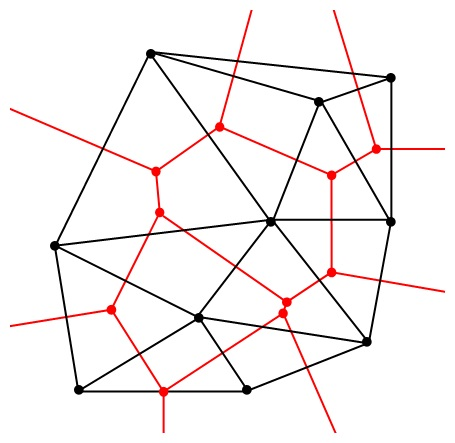
\includegraphics[width=7cm]{Delaunay_Voronoi.jpg}
\caption{The Delaunay triangulation in black is the dual of the Voronoi diagram in red, \cite{Wiki4}.}
\label{fig:Voronoi}
\end{center}
\end{figure}
Delaunay triangulation triangulates the convex hull of $V$ and, therefore it does not constitutes a suitable method for reconstruct the surface formed by a point cloud. 
\\ \indent An important method in surface reconstruction is the $\alpha$-shapes method, \cite{edelsbrunner2010alpha, guo1997surface}. Starting from the Delaunay triangulation $T^\prime$ of a point set $V$, the corresponding $\alpha$-shape of $V$ is formed by the only triangles of $T^\prime$ that satisfy the so-called "$\alpha$-test".
For each triangle we calculate the radius of the circumcircle. If the radius is larger that $\alpha$ the triangle is removed from the shape. The rule of the parameter $\alpha$ is highly significant in this procedure. We would choose $\alpha$ such the better approximation of the shape formed by the points of $V$ is obtained. 
The choice of the parameter $\alpha$ is closely related to the radius of the circumcircles. A possible strategy is to find the radius of the greater empty circumcircle. Thus $\alpha$ is related to the density $\delta$ of the point sets $V$. In particular $\alpha$ is inversely proportional to $\delta$:
\begin{equation}
\alpha=C\frac{1}{\delta}\;,
\end{equation}
with $C$ a constant and $\delta$ is:
\begin{equation}
\delta=\frac{N}{\mbox{surface area}}\; ,
\end{equation}
where $N$ is the number of points in $V$ and the surface area is the area inside the boundaries of the region formed by the points cloud. Hence $\delta$ is given for a fixed point set and the value of $C$ needs to be determined by numerical simulations.
% Insert algorithm
\\
%Let us define a Voronoi diagram in a metric space.
%The simplest case that we can have is the two-dimensional case that is the case where $X=\mathbb{R}^2$.
%The tuple $\mathcal{S}=\{1,\cdots,n\}\subset \mathbb{R}^2$ is now a set of points. The Voronoi diagram of $\mathcal{S}$ is a subsection of $\mathbb{R}^2$ such that every other region around a point $p\in \mathcal{S}$ contains all points that are closer to $p$ than to every point in $\mathcal{S}$. A triangulation of the point set $\mathcal{S}$ is a set of edges $\mathcal{E}$ whose extremes are points of $\mathcal{S}$ such that the faces of each triangle are bounded by three edges and any edge that is not in $\mathcal{E}$ intersects one of the existing edges. The Delaunay triangulation is the dual graph of the Voronoi diagram: it consists of vertices (the points in $\mathcal{S}$) and it has an edge between two vertices if the two corresponding faces share an edge. \\
\indent $\alpha$-shapes are a powerful tool to reconstruct surfaces. However, there exist surfaces that are not described well by $ \alpha $-shapes. Indeed for some surfaces there exist no value of $\alpha$ that includes all desired triangles and deletes all undesired triangles. For example, it can be difficult to obtain a good approximation of a shape formed by a non-uniform points set if the parameter $\alpha$ is determined according to the density of the point cloud. Furthermore, the $\alpha$-shape method does not work well when the shape has a sharp turn or a joint. In this case $\alpha$-shapes often give a "webbed-foot" appearance at such joints since they improperly connect the adjacent surfaces. To overcome this issue, Teichmann and Capps presented an alternative approach to establish the value of $\alpha$, \cite{teichmann1998surface}. Their density-scaled $\alpha$-shapes method constitutes an improvement of "classical" $\alpha$-shapes.
% BRIDGE
There are several ways to determine the value of $\alpha$ \cite{mandal1997selection}; we provide a technique that exploits the conservation of the \'{e}tendue in phase space. The essence of our approach is explained in the following.

%The first step of this method is to make a triangulation of the point cloud.
%Then the key idea is to compute somehow the point-density of each point and use this to get an approximation of the point density of a triangle. In this way one can reduce the $\alpha$-value in areas where the triangle's point density (see equation \ref{delta_t} for the definition) is higher than average in such a way that is possible to obtain a finer level of detail for areas that have an higher density.
%More precisely, each point $ \textbf{p}\in \mathcal{S} $ has a local point density defined as
%\begin{equation}
%\delta (\textbf{p})= \sum_{\textbf{q}\in \mathcal{S}}\Big( 1-\frac{\textrm{d}(q,p)}{\lambda}\Big) \qquad \forall \textbf{q} \mbox{\;\;such that\;\;} \textrm{d}(\textbf{p},\textbf{q})<\lambda\,,
%\end{equation}
%where $ \lambda $ is the constant radius of the local neighborhood and $\textrm{d}(\textbf{x},\textbf{y})$ is the Euclidean distance.
%When local density is larger than the average, that is when
%\begin{equation}
%\delta (\textbf{p}) >\frac{1}{| \mathcal{S} |}\sum_{\textbf{q}\in \mathcal{S}}\delta (\textbf{q})
%\end{equation}
%we know some properties about the region surrounding $\textbf{p}$.
%For instance, if the point set is uniformly distributed then it is possible to find areas with a high-density in the case where there are two closely separated surfaces.  In point sets of non-uniform distribution, high densities are found when the surface presents a joint discontinuity. The algorithm developed by Teichmann and Capps is structured as follow.
%After computing density information for each point they make a triangulation of the point set. Then they calculate the average density  $\delta(t)$ for each triangle $\Delta_{abc}$ defined as:
%\begin{equation}
%\delta(t)=\frac{\delta(a)+\delta(b)+\delta(c)}{3 \mu}\,,
%\label{delta_t}
%\end{equation}
%where $\mu$ is the global average density of the entire point set $\mathcal{S}$.
%If $\delta(t)$ is greater than $1$ the density of the point cloud is higher. Hence is necessary to define another value of $\alpha$:
%\begin{equation}
%\alpha^{\;\prime} = \frac{\alpha}{\delta(t)^\sigma}
%\end{equation} where $\sigma$ is a value that is adjusted by the user.
%If  $\delta$ is less than $1$ the $\alpha$-value is not modified.
%In this way it is possible to have a finer precision on the shape formed by the point set where the density is higher than the average density. Hence it is possible to distinguish two separated objects with different density.

% We want to determine the boundaries in phase space
% Jorg
% It is useful to understand whether the approximation is correct
\section{Determination of $\alpha$ using \'{e}tendue conservation}
As mentioned in Section \ref{sec:PSconcept} \'{e}tendue can be seen as an area in a two-dimensional phase space. 
Therefore, given an optical system with a line segment source $\point{S} = [-\variabile{a}, \variabile{a}]$, the \'{e}tendue at the source coincides with the area of the entire PS \set{S}{}{}, given by:
\begin{equation}\label{eq:etenduesource}
U = 4\n_1 \variabile{a} \sin(\myangle_1^{\textrm{max}})\,,
\end{equation}
 where $\variabile{a}$ is the half length of the source, $\n_1$ the index of refraction of the medium in which the \point{S} is located and $\myangle_1^{\textrm{max}}$ is the maximum value of the angle that the rays make with the normal $\boldsymbol{\nu}_1$ of the source.\\ \indent 
For some optical systems, all the rays emitted by the source arrive to the target, for some others there are also rays that can end up to other detectors. 
The \'{e}tendue of a set of rays is defined by the area they occupy in PS. Indicating with \set{R}{$1$}{}$(\Pi)$ the regions in source PS formed by the rays that reach the target and with \set{R}{}{} the corresponding regions at the target, the \'{e}tendue $U_1$ at source of the rays that reach the target is:
\begin{equation}\label{eq:etenduesumsource}
U_1 = \sum_\Pi{U_1\big(\mbox{\set{R}{$1$}{}}(\Pi)\big)},
\end{equation}
where the sum is over all possible paths $\Pi$ and $U_1\big(\mbox{\set{R}{$1$}{}}(\Pi)\big)$ is the contribution to \'{e}tendue given by the rays inside the region 
\set{R}{$1$}{}$(\Pi)$ in source PS given by:
\begin{equation}\label{eq:etendueintegralsource}
U_1\big(\mbox{\set{R}{$1$}{}}(\Pi)\big) = {\int\!\!\int}_{\emph{R}_1(\Pi)} \textrm{d}\variabile{q}\,\textrm{d}\variabile{p}.
\end{equation}
Similarly the \'{e}tendue at the target of the rays emitted by the source is:
\begin{equation}
U_\textrm{t}= \sum_\Pi{U_\textrm{t}\big(\mbox{\set{R}{}{}}(\Pi)\big)},
\end{equation}
with
\begin{equation}\label{eq:etendueintegraltarget}
U_\textrm{t}\big(\mbox{\set{R}{}{}}(\Pi)\big) = {\int\!\!\int}_{\emph{R}(\Pi)} \textrm{d}\variabile{q}\,\textrm{d}\variabile{p}.
\end{equation}
In order to determine the value of $\alpha$ in the $\alpha$-shape procedure that better approximates the boundaries $\partial$\set{R}{}{}$(\Pi)$ we use \'{e}tendue conservation, i.e. $U_{\textrm{t}}= U_1$ as explianed in the following.\\ \indent
The $\alpha$-shapes method is applied to every region \set{R}{}{}$(\Pi)$ for a range of values of $\alpha$;
   for each value an approximation of the boundaries $\partial$\set{R}{}{}$(\Pi)$ is obtained and
   the intersection points $\variabile{q}^{\textrm{\,max}}(\Pi,\variabile{p})$ and $\variabile{q}^{\textrm{\,min}}(\Pi,\variabile{p})$ between $\partial$\set{R}{}{}$(\Pi)$
and the horizontal lines $\variabile{p}=const$, with $\variabile{p}\in[-1,1]$, are computed for every path $\Pi$.
Therefore Equation (\ref{eq:etendueintegraltarget}) becomes
\begin{equation}\label{eq:etenduetarg}
 U_\textrm{t}\big(\mbox{\set{R}{}{}}(\Pi)\big)= \int_{-1}^{1}{\Big(\variabile{q}^{\textrm{\,max}}(\Pi,\variabile{p})-\variabile{q}^{\textrm{\,min}}(\Pi,\variabile{p})\Big)} \textrm{d}\variabile{q}\,\textrm{d}\variabile{p}.
\end{equation} In case more than two intersection points between line $\variabile{p}=const$ and $\partial$\set{R}{}{}$(\Pi)$ occur, the previous equation needs to be generalized. Suppose that $\variabile{r}$ intersection points $\big(\variabile{q}^{\,\variabile{i}}(\Pi,\variabile{p}), \variabile{p}\big)_{\variabile{i} = 1, \cdots, \variabile{r}}$ are found. 
First their $\variabile{q}$ coordinates are ordered in ascending order, second the target \'{e}tendue is calculated using
\begin{equation}\label{eq:etenduetarg1}
 U_\textrm{t}\big(\mbox{\set{R}{}{}}(\Pi)\big) =\sum_{\variabile{i} = 1}^{\variabile{m}} \int_{-1}^{1}
{(\variabile{q}^{\,2\variabile{i}}(\Pi,\variabile{p})}-{\variabile{q}^{\,2\variabile{i}-1} (\Pi, \variabile{p}) )} \textrm{d}\variabile{q}\,\textrm{d}\variabile{p}\,,
\end{equation}
where $\variabile{m}$ is the integer part of $\variabile{r}/2$ with $\variabile{r}$. 
The integrals in Equation (\ref{eq:etenduetarg}) and (\ref{eq:etenduetarg1}) are calculated discretizing the interval $[-1, 1]$
   into $\nbin=100$ sub-intervals of equal length, the so-called bins, and using the trapezoidal rule to approximate the integral.
   Note that by increasing the value of $\alpha$, the area inside the $\alpha$-shape increases and, consequently, the \'{e}tendue raises.
\\ \indent Eventually, matching the value of the \'{e}tendue at the source $U_1$ with the value of the \'{e}tendue at the target $U_{\textrm{t}}$, a unique value $\alpha_{c}$ of $\alpha$  is determined. Implemented the $\alpha$-shapes procedure with $\alpha = \alpha_c$, the best approximation of the boundaries $\partial$\set{R}{}{}$(\Pi)$ is found and the intensity at the target can be calculated.\\ \indent If two intersection points between $\variabile{p}=const$ and $\partial$\set{R}{}{}$(\Pi)$ are found the target intensity is calculated using Equation ($\ref{eta2}$), otherwise the generalized equation:
\begin{equation}
I_{PS}(\variabile{p}) = \sum_{\Pi, \variabile{i} }\int_{\variabile{q}^{\,2\variabile{i}-1}(\Pi, \variabile{p})}^{\variabile{q}^{\,2\variabile{i}}( \Pi, \variabile{p})}L(\variabile{q}, \variabile{p})\textrm{d}\variabile{q}\,,
\label{eq:Ips}
\end{equation}
where the summation over $\Pi$ is for all the paths $\Pi$ for which the intersection $\variabile{p} = const$ and \set{R}{}{}$(\Pi)$ is not empty, and the summetion over $\variabile{i}$ is for all $\variabile{i} = 1,2, \cdots, \variabile{m}$, and the summation for the path $\Pi$ 
In order to clarify our idea we apply the method to a simple optical system.
\\ \indent Let us consider the two-faceted cup introduced in Chapter \ref{chap:raytracing} and depicted in Figure \ref{fig:cup}. The half length of the source is $\variabile{a}=2$, the maximum angle is $\myangle_1^{\textrm{max}} = \pi/2$ and \point{S} is located in air, i.e. $\n_1=1$. Therefore, the \'{e}tendue $U_1 $ at the source is $U_1=8$. For the two-faceted cup all the rays emitted by \point{S} arrive to \point{T}, hence from \'{e}tendue conservation we obtain that also the target \'{e}tendue $U$ has to be $U = 8$.
For some optical systems, not all the rays emitted by the source arrive to the target.  



% Explain the idea: use etendue conservation
% Do the example for the two faceted cup
% Explain the TIR collimator
\section{Results for a TIR collimator}

\indent
 For the TIR-collimator we considered (Figure \ref{fig:tir}), the area of $\mathcal{P}_\textrm{s}$ is equal to $7.92$, since $a = 4$ and $\sin(t_{max}) ~=~ 0.99$.
 The rays traced are uniformly distributed over $\mathcal{P}_\textrm{s}$, and they cover it almost entirely.
 More precisely, given two adjacent paths $\Pi_i$ and $\Pi_j$, the regions $R_{\textrm{s}, \Pi_i}$ and $R_{\textrm{s}, \Pi_j}$ have usually a common boundary and only small parts of the source do not illuminate the target of the TIR-collimator (see Figure \ref{fig:sourcePS}).
 Indeed a small number of rays reach the left and the right reflectors of our optical system (surfaces $13$ and $15$ in Figure $\ref{fig:tir}$), which are note considered to determine the target intensity.
 As a result, the \'{e}tendue at the source $E_{\textrm{s}}$ can be calculated removing from the area of the entire $\mathcal{P}_\textrm{s}$ those areas occupied by the regions formed by the rays that hit the left and the right detector (white regions in Figure $\ref{fig:tir}$).  Therefore, $E_{\textrm{s}}$ can be approximate by the following relation:
 \begin{equation}
 E_{\textrm{s}}\approx 7.92-2A_{T}
 \end{equation}
 where $A_{T}$ is the approximated area of one of the white regions in Figure $\ref{fig:tir}$ and, it is computed approximating those regions with the area of the triangles shown in Fig. \ref{fig:sourcePS} with black lines.
 %by $E_{\textrm{s}} = 7.68$.
 On the contrary, large parts of the target phase space $\mathcal{P}_{\textrm{t}}$ are not illuminated by any ray and the regions $R_{\textrm{t}, \Pi_j}$ are always disconnected. Hence, the total \'{e}tendue at the target, $E_{\textrm{t}}$, is given by the sum of the \'{e}tendues related to each region $R_{\textrm{t}, \Pi_{j}}$:
 \begin{equation}
 E_{\textrm{t}} = \sum_{j = 1}^p E(R_{\textrm{t}, \Pi_j})\,,
 \end{equation}
 where $E(R_{\textrm{t}, \Pi_j})$ is the contribution to the \'{e}tendue at the target given by the rays inside the region $R_{\textrm{t}, \Pi_j}$. $E(R_{\textrm{t}, \Pi_j})$ is defined by:
  \begin{equation}\label{etenduepartial}
 E(R_{\textrm{t}, \Pi_j}) = {\int\!\!\int}_{R_{\textrm{t}, \Pi_j}} \textrm{d}q\textrm{d}\eta \,.
 \end{equation}
 To calculate the previous integral the $\alpha$-shapes method is applied to the regions
  $R_{\textrm{t},\Pi_j}$ for a range of values for $\alpha$;
   for each value an approximation of the boundaries $\partial R_{\textrm{t},\Pi_j}$ is obtained and
   the intersection points $(q_{\Pi_j,i}( \eta))_{i = 1, \cdots, r}$ between $\partial R_{t,\Pi_j}$
and the horizontal lines $\eta ~=~ const$, with $\eta~\in~[-1,1]$, are computed for each $j \in \{1, \cdots, p\}$.
%When $r=2$, that is only two intersection points occur,
Ordering the points $(q_{\Pi_j,i}( \eta))_{i = 1, \cdots, r}$ in ascending order,
 Equation ($\ref{etenduepartial}$) becomes:
\begin{equation}\label{eq:etenduetarg}
 E(R_{\textrm{t}, \Pi_j}) =\sum_{i = 1}^{m} \int_{-1}^{1}{(q_{\Pi_j, 2i}( \eta)}-{q_{\Pi_j,2i-1} ( \eta) )} \textrm{d}q\textrm{d}\eta \,,
\end{equation}
where $m$ is the integer part of $r/2$ and $r$ is the number of the intersection point between $\partial R_{t,\Pi_j}$
and the horizontal lines $\eta ~=~ const$. The integral in Equation (\ref{eq:etenduetarg}) is calculated discretizing the interval $[-1, 1]$
   into $Nb=100$ sub-intervals of equal width and using the trapezoidal rule to approximate the integral.
   Note that by increasing the value of $\alpha$, the area inside the $\alpha$-shape increases and, consequently, the \'{e}tendue raises.
\noindent Eventually, matching the value of the \'{e}tendue at the source $E_{\textrm{s}}$ with the value of the \'{e}tendue at the target $E_{\textrm{t}}$, a unique value of $\alpha$, $\alpha_{c}$, is determined.
 Figure \ref{fig:etendueTS} shows that a value of $\alpha_c = 0.041$ is obtained for a set of $1.9\cdot 10^4$ rays.
 \begin{figure}[h]
  \begin{center}
  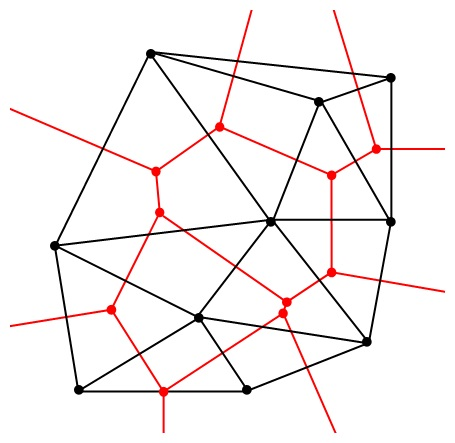
\includegraphics[width=7.7cm]{Delaunay_Voronoi.jpg}
  \end{center}
  \caption{\footnotesize{The source and the target \'{e}tendue are depicted with the dotted red line and the blue line, respectively.
  $E_\textrm{t}$ is computed for a range of values for $\alpha$. $E_{\textrm{s}} \approx 7.68$
   The green dot indicates the value of $\alpha_c = 0.041$ which gives the best approximation of the boundaries $\partial R_{\textrm{t}, \Pi_j}$ at the target.
   Around $1.9 \cdot 10^4$ rays have been traced in PS.
  }}
  \label{fig:etendueTS}
\end{figure}
  \begin{figure}[h]
  \begin{center}
  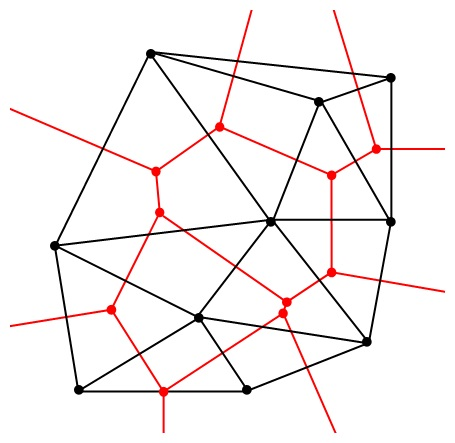
\includegraphics[width=7.7cm]{Delaunay_Voronoi.jpg}
  \end{center}
  \caption{\footnotesize{Target phase space representation of a set of $1.9 \cdot 10^4$ rays.
  The choice of the colors for each path is the same as in Figure $\ref{fig:sourcePS}$.
  Rays that follow the same path are depicted with the same color. The boundaries $(\partial R_{\textrm{t}, \Pi_j})_{j = 1, \cdots, p}$ are computed through the $\alpha$-shapes method with $\alpha = 0.041$.}}
  \label{fig:targetPS}
\end{figure}

 \noindent The $\alpha$-shapes method with $\alpha = \alpha_{c}$ is applied to the target regions $R_{\textrm{t}, \Pi_j}$, and the
 best approximations of the boundaries
 $(\partial R_{\textrm{t}, \Pi_j})_{j = 1, \cdots, p}$ are obtained (see Figure \ref{fig:targetPS}).
\newline \indent To conclude, we compute the target intensity, which is defined in $\mathcal{P}_{\textrm{t}}$ by Equation (\ref{I(eta)}).
From Equation (\ref{luminance}), we obtain:
\begin{equation}
I_{PS}(\eta) = \sum_{ i, j }\int_{q_{\Pi_j,2i-1}( \eta)}^{q_{\Pi_j, 2i}( \eta)}L_\textrm{t}(q, \eta)\textrm{d}q\,,
\label{eq:Ips}
\end{equation}
where the summation for the indexes $i$ is over all $i = 1,2, \cdots, m$, and the summation for the $j$ indexes is over all $j$ for which the intersection between $\eta = const$ and $R_{t, \Pi_j}$ is not empty.






% 
\label{sec:Tir_alpha}

